\section*{Implementation}

\subsection*{Summary of Implementation Progress}
The verifier now supports a complete CHC-based verification flow for Chiron programs: parsing source into IR, extracting user variables and loop counters, constructing symbolic state relations, generating instruction-level transition rules, and checking user properties through Z3 Fixedpoint/SPACER. The core state model includes program counter, turtle coordinates, heading, pen state, user variables, and internal counters, and the tool reports clear verdicts (\texttt{PASSED}, \texttt{FAILED}, \texttt{UNKNOWN}) using a structured return object with timing and per-property outcomes. The verification interface is fully callable through \texttt{CHC\_Verification(...)} and supports robust input validation, controlled property parsing, and consistent result reporting.

In addition to baseline verification, the implementation includes explicit heading-grid safety checking through a dedicated \texttt{BadHeading} relation, configurable scope controls (\texttt{all}, \texttt{terminating}, \texttt{at\_pc}, \texttt{upto\_pc}), and user-selectable hint behavior for performance-vs-assumption tradeoffs. A basic optimization pipeline has been integrated with static turn-safety analysis, repeat-loop summarization, and exact 15-degree trigonometric handling on the heading lattice. To improve usability, a separate semantic helper transpiler was added so readable user-facing helper expressions can be lowered to solver-ready property strings without modifying the core verifier. The implementation is supported by expanded correctness and performance test coverage across modes, scopes, heading behavior, and optimization settings.

\subsection*{Verification Modes and Property Scopes}

\subsubsection*{Verification Modes}
\begin{enumerate}[leftmargin=1.5em, itemsep=4pt, topsep=4pt]
    \item \textbf{\texttt{default}.} Verifies from a single concrete start state: \texttt{pc=0}, \texttt{xcor=0}, \texttt{ycor=0}, \texttt{heading=0}, \texttt{pendown=False}, all user variables initialized to \texttt{0}, and all loop counters initialized to \texttt{0}. This is the baseline configuration for proving invariants from Chiron's standard start state.
    \item \textbf{\texttt{specific}.} Verifies from a concrete parameterized start state. The caller supplies values for user variables through \texttt{params}; any omitted user variable is defaulted to \texttt{0}. The rest of the state remains fixed at the standard start configuration (\texttt{pc=0}, zero position, zero heading, pen up, counters zero).
    \item \textbf{\texttt{universal}.} Verifies over a symbolic family of initial states. The verifier fixes \texttt{pc=0}, \texttt{pendown=True}, and all counters to \texttt{0}; constrains \texttt{heading} to the 15-degree grid; and leaves \texttt{xcor}, \texttt{ycor}, and user variables unconstrained. Optional \texttt{input\_ranges} can additionally restrict selected user variables.
\end{enumerate}

\subsubsection*{Property Scopes}
\begin{enumerate}[leftmargin=1.5em, itemsep=4pt, topsep=4pt]
    \item \textbf{\texttt{all}.} Checks whether the property holds for every reachable state in the verifier's symbolic model, regardless of control location.
    \item \textbf{\texttt{terminating}.} Restricts checking to reachable terminal states, i.e. states whose \texttt{pc} equals the terminal program counter. If the verifier cannot establish reachability of termination, the result is conservatively reported as \texttt{UNKNOWN}.
    \item \textbf{\texttt{at\_pc}.} Restricts checking to reachable states at one exact control point \texttt{pc\_target}. This scope requires an explicit \texttt{pc\_target}; if that program counter is unreachable, the scoped query is returned as \texttt{UNKNOWN}.
    \item \textbf{\texttt{upto\_pc}.} Restricts checking to the reachable execution prefix satisfying \texttt{0 <= pc <= pc\_target}. This is useful for prefix invariants that should hold before or up to a particular program point.
\end{enumerate}

The API also enforces a few scope-specific restrictions: \texttt{pc\_target} is required for \texttt{at\_pc} and \texttt{upto\_pc}, forbidden for \texttt{all} and \texttt{terminating}, and the pc-scoped options are disabled when \texttt{optimization\_level=BASIC} because loop summarization currently targets whole-program or terminal-state reasoning.

\subsubsection*{Optimization Levels}
\begin{enumerate}[leftmargin=1.5em, itemsep=4pt, topsep=4pt]
    \item \textbf{\texttt{OptimizationLevel.NONE}.} Uses the baseline encoding: the verifier emits the standard per-instruction CHC rules and supports all four property scopes (\texttt{all}, \texttt{terminating}, \texttt{at\_pc}, \texttt{upto\_pc}).
    \item \textbf{\texttt{OptimizationLevel.BASIC}.} Enables the current optimization pipeline, namely turn-safety suppression of unnecessary \texttt{BadHeading} rules, repeat-loop summarization, and conditional branch merging inside summarized loop bodies. This level is intended for whole-program or terminal-state reasoning, so the API rejects \texttt{at\_pc} and \texttt{upto\_pc} queries when \texttt{BASIC} is selected.
\end{enumerate}

\subsection*{End-to-End Pipeline View}

Figure~\ref{fig:end_to_end_pipeline} shows the full safety-verification flow from the Chiron CLI and Python entrypoints into the core CHC engine, including fixedpoint construction, optimization-aware rule emission, semantic gates, and structured result reporting.
\begin{figure}[h]
\centering
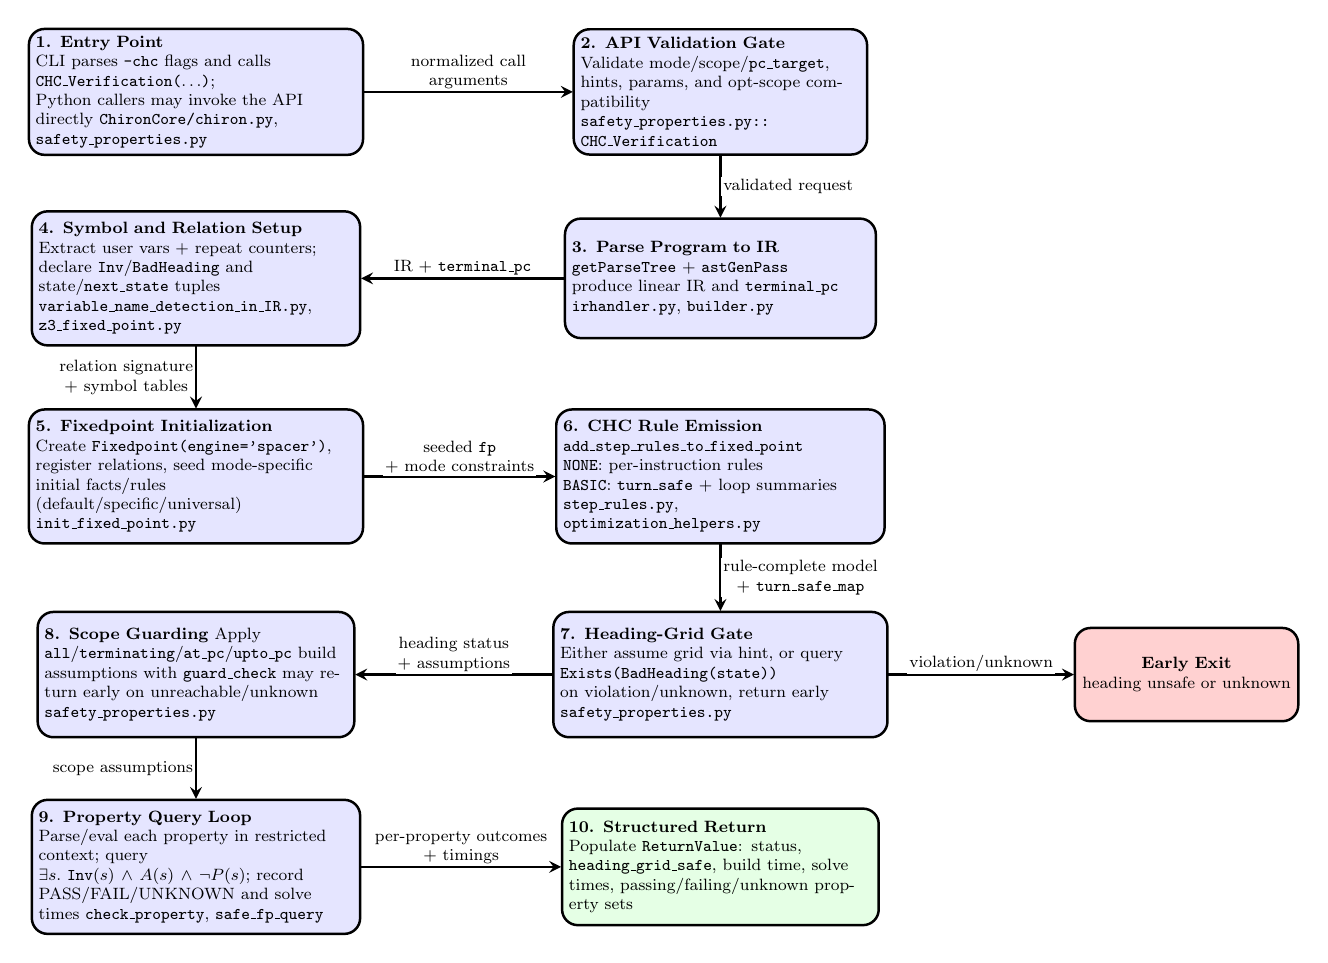
\begin{tikzpicture}[>=stealth, line width=0.9pt, font=\footnotesize, scale=0.74, transform shape]

\node[draw, rounded corners=2mm, align=left, text width=5.5cm, minimum height=1.95cm, fill=blue!10] (p1) at (0,0)
{\textbf{1. Entry Point}\\
CLI parses \texttt{-chc} flags and calls
\texttt{CHC\_Verification($\ldots$)};\\
Python callers may invoke the API directly
\texttt{ChironCore/chiron.py}, \texttt{safety\_properties.py}};

\node[draw, rounded corners=2mm, align=left, text width=4.8cm, minimum height=2.15cm, fill=blue!10] (p2) at (9.0,0)
{\textbf{2. API Validation Gate}\\
Validate mode/scope/\texttt{pc\_target},\\
hints, params, and opt-scope compatibility\\
\texttt{safety\_properties.py::\\CHC\_Verification}};

\node[draw, rounded corners=2mm, align=left, text width=5.1cm, minimum height=2.05cm, fill=blue!10] (p3) at (9.0,-3.2)
{\textbf{3. Parse Program to IR}\\
\texttt{getParseTree} + \texttt{astGenPass}\\
produce linear IR and \texttt{terminal\_pc}\\
\texttt{irhandler.py}, \texttt{builder.py}};

\node[draw, rounded corners=2mm, align=left, text width=5.4cm, minimum height=2.30cm, fill=blue!10] (p4) at (0,-3.2)
{\textbf{4. Symbol and Relation Setup}\\
Extract user vars + repeat counters;\\
declare \texttt{Inv}/\texttt{BadHeading} and\\
state/\texttt{next\_state} tuples\\
\texttt{variable\_name\_detection\_in\_IR.py},\\
\texttt{z3\_fixed\_point.py}};

\node[draw, rounded corners=2mm, align=left, text width=5.5cm, minimum height=2.30cm, fill=blue!10] (p5) at (0,-6.6)
{\textbf{5. Fixedpoint Initialization}\\
Create \texttt{Fixedpoint(engine='spacer')},\\
register relations, seed mode-specific\\
initial facts/rules \\(default/specific/universal)\\
\texttt{init\_fixed\_point.py}};

\node[draw, rounded corners=2mm, align=left, text width=5.4cm, minimum height=2.30cm, fill=blue!10] (p6) at (9.0,-6.6)
{\textbf{6. CHC Rule Emission}\\
\texttt{add\_step\_rules\_to\_fixed\_point}\\
\texttt{NONE}: per-instruction rules\\
\texttt{BASIC}: \texttt{turn\_safe} + loop summaries\\
\texttt{step\_rules.py}, \texttt{optimization\_helpers.py}};

\node[draw, rounded corners=2mm, align=left, text width=5.5cm, minimum height=2.15cm, fill=blue!10] (p7) at (9.0,-10.0)
{\textbf{7. Heading-Grid Gate}\\
Either assume grid via hint, or query\\
\texttt{Exists(BadHeading(state))}\\
on violation/unknown, return early\\
\texttt{safety\_properties.py}};

\node[draw, rounded corners=2mm, align=center, text width=3.6cm, minimum height=1.6cm, fill=red!18] (p7exit) at (17.0,-10.0)
{\textbf{Early Exit}\\
heading unsafe or unknown};

\node[draw, rounded corners=2mm, align=left, text width=5.2cm, minimum height=2.15cm, fill=blue!10] (p8) at (0,-10.0)
{\textbf{8. Scope Guarding}
Apply \texttt{all}/\texttt{terminating}/\texttt{at\_pc}/\texttt{upto\_pc}
build assumptions with \texttt{guard\_check}
may return early on unreachable/unknown
\texttt{safety\_properties.py}};

\node[draw, rounded corners=2mm, align=left, text width=5.4cm, minimum height=2.30cm, fill=blue!10] (p9) at (0,-13.3)
{\textbf{9. Property Query Loop}\\
Parse/eval each property in restricted context;
query\\ \(\exists s.\ \texttt{Inv}(s)\land A(s)\land \neg P(s)\);
record PASS/FAIL/UNKNOWN and solve times
\texttt{check\_property}, \texttt{safe\_fp\_query}};

\node[draw, rounded corners=2mm, align=left, text width=5.2cm, minimum height=2.00cm, fill=green!10] (p10) at (9.0,-13.3)
{\textbf{10. Structured Return}\\
Populate \texttt{ReturnValue}: status,
\texttt{heading\_grid\_safe}, build time, solve times,
passing/failing/unknown property sets};

\draw[->] (p1.east) -- node[above, align=center, fill=white, inner sep=1pt] {normalized call\\arguments} (p2.west);
\draw[->] (p2.south) -- node[right, align=center, fill=white, inner sep=1pt] {validated request} (p3.north);
\draw[->] (p3.west) -- node[above, align=center, fill=white, inner sep=1pt] {IR + \texttt{terminal\_pc}} (p4.east);
\draw[->] (p4.south) -- node[left, align=center, fill=white, inner sep=1pt] {relation signature\\+ symbol tables} (p5.north);
\draw[->] (p5.east) -- node[above, align=center, fill=white, inner sep=1pt] {seeded \texttt{fp}\\+ mode constraints} (p6.west);
\draw[->] (p6.south) -- node[right, align=center, fill=white, inner sep=1pt] {rule-complete model\\+\ \texttt{turn\_safe\_map}} (p7.north);
\draw[->] (p7.east) -- node[above, align=center, fill=white, inner sep=1pt] {violation/unknown} (p7exit.west);
\draw[->] (p7.west) -- node[above, align=center, fill=white, inner sep=1pt] {heading status\\+ assumptions} (p8.east);
\draw[->] (p8.south) -- node[left, align=center, fill=white, inner sep=1pt] {scope assumptions} (p9.north);
\draw[->] (p9.east) -- node[above, align=center, fill=white, inner sep=1pt] {per-property outcomes\\+ timings} (p10.west);
\end{tikzpicture}
\caption{End-to-end safety verification pipeline from CLI/API entry to CHC construction, solver querying, and result delivery. Each stage is annotated with its primary file-level owner.}
\label{fig:end_to_end_pipeline}
\end{figure}

\subsection*{File-wise Implementation Details}
\textbf{1. \texttt{CHC-Verification/variable\_name\_detection\_in\_IR.py}}
Extracts user variables and internal repeat counters from linear IR. Also defines optimization-level controls that are consumed during CHC generation.
Variable extraction uses recursive AST traversal through \texttt{parse\_variables\_from\_ir\_expr()} and \texttt{parse\_variables\_from\_ir\_cond()}, producing a \texttt{symbol\_table} of user-declared variables and a \texttt{counter\_table} of loop iteration variables.
These two tables determine the arity and argument ordering of the \texttt{Inv} relation declared in the next stage, so the accuracy of extraction directly governs the completeness of the symbolic state model.

\textbf{2. \texttt{CHC-Verification/z3\_fixed\_point.py}}
Builds the mode-aware state signature and declares core relations such as \texttt{Inv} and \texttt{BadHeading}. This module defines the relation arity and state-vector shape used by downstream rules.
The full state vector carries program counter, turtle coordinates (\texttt{xcor}, \texttt{ycor}), heading, pen state, all user variables, and all loop counters; both a \emph{current-state} and a \emph{next-state} copy are constructed so transition rules can be expressed as implications between them.
\texttt{BadHeading} shares the same state-vector shape as \texttt{Inv}, allowing heading-violation rules to reuse the same variable symbols and be registered in the same fixedpoint context without duplicating infrastructure.

\textbf{3. \texttt{CHC-Verification/init\_fixed\_point.py}}
Initializes the Z3 Fixedpoint context (SPACER engine), registers relations, and seeds base constraints according to verification mode (\texttt{default}, \texttt{specific}, \texttt{universal}).
In \texttt{default} mode the initial fact pins all state components to concrete values (\texttt{pc=0}, coordinates zero, heading zero, pen up, all variables zero); in \texttt{universal} mode coordinates and user variables are left unconstrained while heading is restricted to the 15-degree grid and pen is forced down, capturing the widest possible input class.
The \texttt{specific} mode accepts a caller-supplied parameter dictionary, initializes the corresponding user variables to those concrete values, defaults omitted user variables to zero, and keeps the remaining state at the standard start configuration. This enables targeted property checking from a concrete parameterized initial state.
The same module also normalizes and validates \texttt{input\_ranges} for universal mode. A variable may be given as a fixed integer, a closed integer interval \texttt{(lo, hi)}, or \texttt{None} to leave it unconstrained; unknown variable names, non-integer bounds, and malformed ranges are rejected eagerly before any CHC rules are emitted.

\textbf{4. \texttt{CHC-Verification/step\_rules.py}}
Translates each IR instruction into CHC transition rules. It covers assignments, conditionals, movement, heading updates, pen-state updates, assertions, and control-flow jumps. This module is also where optimization-aware rule paths and loop summarization hooks are integrated.
For movement instructions, the rule encodes exact integer arithmetic for heading multiples of 15 degrees by consulting the precomputed trigonometric table in \texttt{optimization\_helpers.py}, avoiding floating-point imprecision in the symbolic encoding.
In \texttt{BASIC} optimization mode, loops that pass the summarizability check are replaced by a single aggregate transition via \texttt{summarize\_loop\_effect()}, reducing the clause count submitted to SPACER and improving convergence on loop-heavy programs while leaving non-summarizable fragments on the standard per-instruction path.
Assertions are encoded as hard safety obligations rather than advisory checks: for an \texttt{AssertCommand}, the true branch advances normally, while the false branch implies \texttt{False} in the fixedpoint system. This turns assertion failure directly into reachability of an inconsistent state, so violated assertions are handled by the same CHC safety machinery as user-supplied properties.

\textbf{5. \texttt{CHC-Verification/safety\_properties.py}}
Implements the top-level API \texttt{CHC\_Verification(...)}. It validates inputs, parses hints, applies scope guards, checks heading-grid safety, evaluates user properties, and returns structured outcomes.
Each user property is evaluated inside an \texttt{eval()} context populated with the current Z3 state variables, so property strings can reference program variables by name without requiring the caller to import Z3 directly.
The return object \texttt{ReturnValue} bundles an overall verdict (\texttt{SUCCESS}, \texttt{ERROR}, or \texttt{UNKNOWN}), a separate \texttt{heading\_grid\_safe} field, wall-clock build and solve timings, and three property lists (\texttt{passing}, \texttt{failing}, \texttt{unknown}).
This module also contains a small robustness layer around SPACER queries. The helper \texttt{safe\_fp\_query()} retries a query with \texttt{spacer.native\_mbp=False} when Z3 raises the known \texttt{mbp to-real} exception on mixed Int/Real reasoning, and \texttt{guard\_check()} proactively disables native MBP before reachability checks. This does not change the logical encoding, but it makes the verifier materially more stable on geometry-heavy benchmarks.

\textbf{6. \texttt{CHC-Verification/heading\_grid.py}}
Defines heading-lattice predicates used to prove or assume 15-degree grid safety.
The core function \texttt{heading\_on\_grid()} generates a Z3 disjunction over all 24 valid headings ($0^\circ, 15^\circ, \ldots, 345^\circ$), which is embedded directly as a guard in movement and turn transition rules rather than checked separately.
This predicate is also the conclusion of the \texttt{BadHeading} violation rules: any transition that produces a heading outside the grid implies \texttt{BadHeading} on the resulting state, allowing SPACER to derive a reachability witness if the invariant is broken.

\textbf{7. \texttt{CHC-Verification/optimization\_helpers.py}}
Implements static turn-safety reasoning, repeat-loop detection, summarizability checks, and exact 15-degree trig tables used by optimized rule generation.
The precomputed \texttt{\_MULT15\_VALUES} dictionary maps each of the 24 valid headings to decimals \(\Delta x\) and \(\Delta y\) displacements scaled, so movement rules submitted to SPACER contain only integer arithmetic other than $xcor$ and $ycor$ update.
The \texttt{is\_summarizable\_loop\_nested()} predicate enforces structural constraints - a positive constant loop bound within \texttt{MAX\_SUMMARIZE\_ITERATIONS}, no \texttt{AssertCommand} nodes, only unit jumps except for supported if/else shapes, and no use of the loop counter inside the body (already summarized inner loops are treated as atomic) - so that the summarization in \texttt{step\_rules.py} is provably sound: every concrete execution through the loop is covered by the emitted summary transition.

\textbf{8. \texttt{CHC-Verification/semantic\_properties.py}}
Provides a user-facing helper-string transpilation layer that lowers readable semantic helpers into raw CHC-compatible property expressions without modifying the core verifier.
Helper functions such as \texttt{is\_nonnegative(v)}, \texttt{position\_in\_box(...)}, \texttt{pen\_is\_up()}, and \texttt{relation\_guarded(...)} are resolved before the property string reaches \texttt{eval()}, so the caller can write human-readable specifications that are automatically converted to Z3 Boolean expressions over state variables.
The companion entry point \texttt{CHC\_Verification\_semantic()} wraps \texttt{CHC\_Verification()} with this transpilation step, keeping the semantic helper layer fully optional and backward-compatible with callers that already supply raw Z3 expressions.

\subsection*{Design Choices}

\begin{enumerate}[leftmargin=1.5em, itemsep=6pt, topsep=4pt]
    \item \textbf{CHCs solved by Z3 SPACER.}
    The verifier encodes program behavior as Constrained Horn Clauses and submits them to Z3's \texttt{Fixedpoint} with \texttt{engine='spacer'}, an IC3/PDR-style Horn-clause solver that performs inductive invariant synthesis.
    \begin{itemize}[leftmargin=1.5em, noitemsep, topsep=2pt]
        \item \noindent\textit{\small \texttt{Benefit:}} Supports unbounded safety checking; returns a concrete counterexample witness on violation, not just a yes/no answer.
        \item \noindent\textit{\small \texttt{Tradeoff:}} Performance is sensitive to nonlinear arithmetic obligations; complex programs or unconstrained inputs can produce \texttt{UNKNOWN} within the timeout.
    \end{itemize}
    \item \textbf{Single global invariant relation \texttt{Inv(pc, xcor, ycor, heading, pendown, vars, counters)}.}
    Full control-and-data state is captured in one unified relation shared across initialization, all transition rules, and every property query.
    \begin{itemize}[leftmargin=1.5em, noitemsep, topsep=2pt]
        \item \noindent\textit{\small \texttt{Benefit:}} \texttt{pc} governs control-flow and termination, geometric variables support spatial predicates, and loop counters make repeat semantics explicit without unrolling; all pipeline stages have this signature.
        \item \noindent\textit{\small \texttt{Tradeoff:}} Properties over a strict variable subset still incur full-arity SPACER reasoning; adding any new state component requires regenerating the entire relation signature and all registered rules.
    \end{itemize}
    \item \textbf{Strict heading lattice with explicit \texttt{BadHeading} relation.}
    Heading is restricted to $\{0^\circ, 15^\circ, \ldots, 345^\circ\}$ and movement arithmetic is handled via a precomputed 24-entry fractional lookup table rather than transcendental \texttt{sin}/\texttt{cos} constraints.
    \begin{itemize}[leftmargin=1.5em, noitemsep, topsep=2pt]
        \item \noindent\textit{\small \texttt{Benefit:}} Keeps all arithmetic linear, with only \texttt{xcor} and \texttt{ycor} as decimals, others as integer, which SPACER handles reliably; heading violations are a first-class proof obligation rather than a silent assumption.
        \item \noindent\textit{\small \texttt{Tradeoff:}} The disjunctive heading guard expands CHC clause size proportionally to the number of valid headings; failing to prove grid preservation yields a conservative \texttt{UNKNOWN} on all downstream property checks.
    \end{itemize}
\end{enumerate}

\subsection*{Optimisations}
\noindent\textit{\small Files: \texttt{CHC-Verification/optimization\_helpers.py}, \texttt{CHC-Verification/step\_rules.py}}

The following optimisations are implemented at \texttt{OptimizationLevel.BASIC} to reduce the number and complexity of CHC rules submitted to SPACER, improving performance on loop-heavy programs and those with many turn instructions while preserving soundness. 

\subsubsection*{Heading Check Optimisation}
\begin{figure}[h]
\centering
\begin{tikzpicture}[>=stealth, line width=0.9pt, font=\footnotesize, scale=0.78, transform shape]
\tikzset{
    hcstage/.style={draw, rounded corners=2mm, align=left, text width=7.2cm, minimum height=1.1cm, fill=blue!10},
    hcdec/.style={draw, diamond, aspect=2.2, align=center, inner sep=2pt, fill=orange!14, minimum width=2.4cm, minimum height=1.0cm},
    hcyes/.style={draw, rounded corners=2mm, align=center, text width=3.4cm, minimum height=1.1cm, fill=green!12},
    hcno/.style={draw, rounded corners=2mm, align=center, text width=3.4cm, minimum height=1.1cm, fill=red!8}
}
\node[hcstage] (h1) at (4.5,0)
{\textbf{1. Data-flow pass over IR}\\
Worklist propagates \texttt{env\_in[i]}: maps variable names to \texttt{True} if provably a multiple of 15.};

\node[hcstage] (h2) at (4.5,-1.9)
{\textbf{2. Transfer function per assignment}\\
\texttt{:v = expr} sets \texttt{env\_out[v] = True} iff \texttt{is\_multiple\_of\_15(expr, env\_in)} is \texttt{True}; clears otherwise.};

\node[hcstage] (h3) at (4.5,-3.8)
{\textbf{3. Join at merge points}\\
\texttt{join\_envs}: keep only keys that are \texttt{True} in \emph{all} incoming \texttt{env\_out} sets.};

\node[hcstage] (h4) at (4.5,-5.7)
{\textbf{4. Check each turn instruction}\\
For \texttt{left}/\texttt{right}: evaluate \texttt{is\_multiple\_of\_15(delta, env\_in[i])}.};

\node[hcdec] (d1) at (4.5,-7.4)
{\textbf{result}\\ \textbf{= True?}};

\node[hcyes] (hy) at (1.2,-9.2)
{\texttt{turn\_safe\_map[i] = True}\\[-1pt]
Skip \texttt{BadHeading}\\[-1pt]
rule for turn $i$.};

\node[hcno]  (hn) at (7.8,-9.2)
{\texttt{turn\_safe\_map[i] = False}\\[-1pt]
Emit \texttt{BadHeading}\\[-1pt]
rule for turn $i$.};

\draw[->] (h1.south) -- (h2.north);
\draw[->] (h2.south) -- (h3.north);
\draw[->] (h3.south) -- (h4.north);
\draw[->] (h4.south) -- (d1.north);
\draw[->] (d1.south west) -- node[above, sloped, fill=white, inner sep=1pt]{\scriptsize yes} (hy.north);
\draw[->] (d1.south east) -- node[above, sloped, fill=white, inner sep=1pt]{\scriptsize no}  (hn.north);
\end{tikzpicture}
\caption{Turn-safe heading inference: data-flow analysis that marks turn instructions whose delta is statically provable as a multiple of 15.}
\label{fig:opt_heading}
\end{figure}

Each turn instruction (\texttt{left}/\texttt{right}) in the standard encoding generates a \texttt{BadHeading} CHC rule asserting that the resulting heading might leave the grid. The heading-check optimisation eliminates these rules wherever the turn amount is statically proven to be a multiple of 15.
\begin{enumerate}[leftmargin=1.5em, noitemsep, topsep=2pt]
    \item A forward data-flow analysis (\texttt{compute\_env\_in}) propagates, for each program point, the set of variables known to hold a multiple-of-15 value. The transfer function \texttt{transfer\_env} updates this set on assignments: if the right-hand side evaluates to \texttt{True} under \texttt{is\_multiple\_of\_15}, the left-hand variable is added; otherwise it is removed.
    \item At merge points (after conditionals), \texttt{join\_envs} takes the intersection — a variable is kept only if it is provably a multiple of 15 on \emph{every} incoming path, preserving soundness across branches.
    \item \texttt{is\_multiple\_of\_15} handles numeric literals (\texttt{n \% 15 == 0}), variable lookups, unary minus, sums and differences (both operands must be known), and multiplication (either factor must be known). Any unsupported shape returns \texttt{None} (unknown), triggering conservative \texttt{BadHeading} emission.
    \item If a turn's delta resolves to \texttt{True} at its program point, \texttt{turn\_safe\_map[i]} is set and the \texttt{BadHeading} rule for that instruction is suppressed, reducing the clause count submitted to SPACER.
\end{enumerate}
\newpage
\subsubsection*{Loop Optimisation}

\begin{figure}[h]
\centering
\begin{tikzpicture}[>=stealth, line width=0.9pt, font=\footnotesize, scale=0.78, transform shape]
\tikzset{
    lstage/.style={draw, rounded corners=2mm, align=left, text width=7.5cm, minimum height=1.1cm, fill=blue!10},
    ldec/.style={draw, diamond, aspect=2.5, align=center, inner sep=2pt, fill=orange!14, minimum width=2.6cm, minimum height=1.0cm},
    lyes/.style={draw, rounded corners=2mm, align=left, text width=7.5cm, minimum height=1.1cm, fill=green!12},
    lno/.style={draw, rounded corners=2mm, align=center, text width=3.2cm, minimum height=1.0cm, fill=red!8}
}
\node[lstage] (l1) at (4.5,0)
{\textbf{1. Detect repeat-loop patterns} (\texttt{find\_repeat\_loops})\\
Match IR pattern: counter init $\to$ guard $\to$ body $\to$ decrement $\to$ back-jump.};

\node[lstage] (l2) at (4.5,-1.9)
{\textbf{2. Sort loops innermost-first}\\
Order by span (\texttt{exit\_idx - init\_idx}); process inner loops before outer to enable nested composition.};

\node[ldec] (d1) at (4.5,-3.6)
{\textbf{summarizable?}};

\node[lno] (ln) at (9.2,-3.6)
{Use per-instruction CHC rules (standard path).};

\node[lyes] (ly) at (4.5,-5.5)
{\textbf{3. Summarize} (\texttt{summarize\_loop\_effect\_nested})\\
Unroll body $N$ times symbolically; compose state deltas with Z3 substitution for inner loops already summarized.};

\node[lstage] (l3) at (4.5,-7.4)
{\textbf{4. Emit single summary rule}\\
\texttt{Inv(init\_pc, s) $\Rightarrow$ Inv(exit\_pc, s')}; collect any \texttt{BadHeading} side-conditions per iteration.};

\node[lstage] (l4) at (4.5,-9.3)
{\textbf{5. Mark skip\_indices}\\
All instructions from \texttt{init\_idx} to \texttt{back\_idx} are skipped during the main IR scan.};

\draw[->] (l1.south) -- (l2.north);
\draw[->] (l2.south) -- (d1.north);
\draw[->] (d1.east) -- node[above, fill=white, inner sep=1pt]{\scriptsize no} (ln.west);
\draw[->] (d1.south) -- node[right, fill=white, inner sep=1pt]{\scriptsize yes} (ly.north);
\draw[->] (ly.south) -- (l3.north);
\draw[->] (l3.south) -- (l4.north);
\end{tikzpicture}
\caption{Repeat-loop summarization: innermost-first pattern matching, summarizability check, symbolic unrolling, and single-rule emission.}
\label{fig:opt_loop}
\end{figure}

Instead of emitting one CHC rule per instruction for every iteration of a \texttt{repeat} loop, the loop optimisation compiles the entire loop into a single transition from loop entry to loop exit.
\begin{enumerate}[leftmargin=1.5em, noitemsep, topsep=2pt]
    \item \texttt{find\_repeat\_loops} scans the IR for the canonical 6-instruction repeat pattern: counter initialisation, a \texttt{counter > 0} guard, a loop body, a \texttt{counter = counter - 1} decrement, and a back-jump. This pattern is produced deterministically by Chiron's parser.
    \item \texttt{is\_summarizable\_loop\_nested} checks structural preconditions: the loop count must be a positive integer not exceeding \texttt{MAX\_SUMMARIZE\_ITERATIONS} (150), the body must contain no \texttt{AssertCommand} nodes, and every non-conditional instruction must have unit jump offset. Already-summarized inner loops are treated as opaque atomic blocks during this check.
    \item Loops are processed innermost-first. \texttt{summarize\_loop\_effect\_nested} unrolls the body $N$ times symbolically, carrying a running Z3 state expression rather than adding solver variables. When an inner loop is encountered, its pre-computed state transformation is applied via Z3 \texttt{substitute} rather than stepping through its instructions again.
    \item The result is one \texttt{fp.rule(ForAll(vars, Inv(init\_pc,~s) $\Rightarrow$ Inv(exit\_pc,~s')))} rule replacing the entire loop, plus any \texttt{BadHeading} side-condition rules accumulated during unrolling. All instructions within the summarized range are added to \texttt{skip\_indices} and bypassed in the main IR scan.
\end{enumerate}

\subsubsection*{Conditional Optimisation}

\begin{figure}[h]
\centering
\begin{tikzpicture}[>=stealth, line width=0.9pt, font=\footnotesize, scale=0.78, transform shape]
\tikzset{
    cstage/.style={draw, rounded corners=2mm, align=left, text width=7.8cm, minimum height=1.1cm, fill=blue!10},
    cdec/.style={draw, diamond, aspect=2.5, align=center, inner sep=2pt, fill=orange!14, minimum width=2.8cm, minimum height=1.0cm},
    cfast/.style={draw, rounded corners=2mm, align=left, text width=3.6cm, minimum height=1.0cm, fill=green!12},
    csym/.style={draw, rounded corners=2mm, align=left, text width=7.8cm, minimum height=1.1cm, fill=purple!8},
    cmerge/.style={draw, rounded corners=2mm, align=left, text width=7.8cm, minimum height=1.1cm, fill=green!12}
}
\node[cstage] (c1) at (4.5,0)
{\textbf{1. Encounter \texttt{ConditionCommand} during segment execution}\\
Check shape: parser-emitted skip-\texttt{BoolFalse} goto or structured if/else.};

\node[cdec] (d1) at (4.5,-1.8)
{\textbf{cond}\\ \textbf{static?}};

\node[cfast] (ctrue)  at (0.9,-3.6)
{Cond \texttt{True}:\\[-2pt]
execute then-branch only, skip else.};

\node[cfast] (cfalse) at (8.0,-3.6)
{Cond \texttt{False}:\\[-2pt]
execute else-branch only, skip then.};

\node[csym] (c2) at (4.5,-5.5)
{\textbf{2. Symbolic execution of both branches}\\
Then: recurse on \texttt{[idx+1, goto\_idx-1]} with guard \texttt{And(pg, cond)}.\\
Else: recurse on \texttt{[false\_start, join\_idx-1]} with guard \texttt{And(pg, Not(cond))}.};

\node[cstage] (c3) at (4.5,-7.5)
{\textbf{3. Merge per state component} (\texttt{\_merge\_branch\_value})\\
If \texttt{then\_j.eq(else\_j)}: keep common value unchanged (no ITE needed).};

\node[cdec] (d2) at (4.5,-9.3)
{\textbf{common}\\ \textbf{add prefix?}};

\node[cfast] (cf1) at (1.2,-11.1)
{Factor: \texttt{base + If(c, a, b)}.};
\node[cfast] (cf2) at (7.8,-11.1)
{Emit: \texttt{If(cond, then\_j, else\_j)}.};

\node[cstage] (c4) at (4.5,-13.5)
{\textbf{4. Merged state continues as single symbolic expression}\\
Merged \texttt{no\_pc} tuple propagated to next instruction; \texttt{BadHeading} side-conditions from both branches collected.};

\draw[->] (c1.south) -- (d1.north);
\draw[->] (d1.south west) -- node[above, sloped, fill=white, inner sep=1pt]{\scriptsize true}  (ctrue.north);
\draw[->] (d1.south east) -- node[above, sloped, fill=white, inner sep=1pt]{\scriptsize false} (cfalse.north);
\draw[->] (d1.south)      -- node[right,  fill=white, inner sep=1pt]{\scriptsize unknown} (c2.north);
\draw[->] (c2.south) -- (c3.north);
\draw[->] (c3.south) -- (d2.north);
\draw[->] (d2.south west) -- node[above, sloped, fill=white, inner sep=1pt]{\scriptsize yes} (cf1.north);
\draw[->] (d2.south east) -- node[above, sloped, fill=white, inner sep=1pt]{\scriptsize no}  (cf2.north);
\draw[->] (cf1.south) -- ++(0,-0.4) -| (c4.north);
\draw[->] (cf2.south) -- ++(0,-0.4) -| (c4.north);
\end{tikzpicture}
\caption{Conditional handling inside summarized loop bodies: static branch elimination and ITE merging with common-prefix factoring.}
\label{fig:opt_cond}
\end{figure}

When a loop body contains if/else branches, the summarizer must represent both paths as a single symbolic state expression rather than splitting into multiple CHC rules.
\begin{enumerate}[leftmargin=1.5em, noitemsep, topsep=2pt]
    \item \texttt{\_execute\_segment\_with\_branch\_merge} handles two conditional shapes produced by Chiron's parser: a \texttt{BoolFalse} skip-goto (used to jump over the else block at the end of the then-branch), and a full structured if/else with a true-branch terminator goto followed by the else block.
    \item If the branch condition is statically \texttt{True} or \texttt{False} at summarization time (Z3's \texttt{is\_true}/\texttt{is\_false}), the dead branch is dropped entirely and no \texttt{If}-expression is introduced, keeping the resulting CHC rule compact.
    \item For the general case, both branches are executed symbolically under their respective path guards (\texttt{And(pg, cond)} and \texttt{And(pg, Not(cond))}), and each state component is merged independently using \texttt{\_merge\_branch\_value}.
    \item \texttt{\_merge\_branch\_value} first checks if then and else values are syntactically equal (\texttt{then\_j.eq(else\_j)}); if so, the common value is kept unchanged without any \texttt{If}. Otherwise it looks for a common additive prefix: \texttt{If(c, base+a, base+b)} is rewritten to \texttt{base + If(c, a, b)}, reducing expression depth in branch-heavy loops. If neither shortcut applies, a plain \texttt{If(cond, then\_j, else\_j)} is emitted.
    \item \texttt{BadHeading} side-conditions accumulated in both branches are collected and emitted together with the summary rule, so heading-grid obligations inside conditional bodies are not lost.
\end{enumerate}

\subsection*{Hints}
\noindent\textit{\small File: \texttt{CHC-Verification/safety\_properties.py}}

Hints are optional caller-supplied strings passed via the \texttt{hints} parameter that let the user trade a proof obligation for an assumption, skipping a solver query when the property is already known to hold. All hints are validated at API entry against the \texttt{Hints} enum; an unrecognised value is rejected before any solving begins.

\begin{itemize}[leftmargin=1.5em, noitemsep, topsep=4pt]
    \item \textbf{\texttt{check\_heading\_always\_on\_grid}} (default). Proves that the turtle's heading stays on the 15-degree grid by querying \texttt{BadHeading}. The result is stored in \texttt{ReturnValue.heading\_grid\_safe}; if the check fails or is unknown, the verifier stops before evaluating user properties.

    \item \textbf{\texttt{heading\_on\_grid\_always}}. Assumes the heading invariant rather than proving it. The \texttt{BadHeading} query is skipped and \texttt{heading\_on\_grid(state[3])} is added directly as an assumption. Useful when all turns are provably multiples of~15 by construction, saving one SPACER call.

    \item \textbf{\texttt{check\_termination}} (default). When \texttt{property\_scope="terminating"}, first queries whether the terminal PC is reachable before checking properties there. If SPACER cannot confirm termination, the run returns \texttt{UNKNOWN} without attempting the property checks.

    \item \textbf{\texttt{always\_terminates}}. Skips the termination reachability check and assumes the terminal state is reachable, adding the terminal-PC guard directly as an assumption. Appropriate for programs with only finite \texttt{repeat} loops and no infinite branches.
\end{itemize}

The two heading hints and the two termination hints form mutually exclusive pairs: supplying both members of a pair is rejected at validation since one proves and the other assumes the same property.
